\documentclass[a4paper,12pt]{article}
\usepackage{graphicx}
\usepackage{verbatim}
\usepackage{amsmath}
\usepackage{enumitem}
\usepackage{tikz}
\usetikzlibrary{arrows, positioning}
\begin{document}
	\title{\textbf{Homework 3}}
	\author{Rostagno 295706}
	\date{\today}
	\maketitle
	
	\centering \textbf{Esercizio 1}\\
	\begin{itemize}
		\item \textbf{Punto a: }
		Per calcolare la funzione di best response di ciascun giocatore \( i \), dobbiamo massimizzare \( u_i(x) \) rispetto a \( x_i \), mantenendo fissati gli \( x_j \) con \( j \neq i \).\\
		Calcoliamo la derivata parziale di \( u_i(x) \) rispetto a \( x_i \):
		\[
		\frac{\partial u_i(x)}{\partial x_i} = -x_i + c_i + \beta \sum_{j \neq i} W_{ij} x_j.
		\]
		Imponiamo che la derivata parziale sia uguale a zero per trovare il punto critico:
		\[
		-x_i + c_i + \beta \sum_{j \neq i} W_{ij} x_j = 0
		\]
		Risolvendo per \( x_i \):
		\[
		x_i = c_i + \beta \sum_{j \neq i} W_{ij} x_j.
		\]
		La funzione di best response per il giocatore \( i \) è:
		\[
		B_i(x_{-i}) = c_i + \beta \sum_{j \neq i} W_{ij} x_j
		\]
		\item \textbf{Punto b: } 
		Dalle slide possiamo scrivere in forma matriciale la condizione per l'equilibrio di Nash:\\
		\[
		x^* = c + \beta W x^*
		\]
		dove $x^*$ é la configurazione dell'equilibrio di Nash\\
		Risolviamo per \( x^* \):
		\[
		(I - \beta W)x^* = c \quad \implies \quad x^* = (I - \beta W)^{-1}c
		\]
		a patto che \( (I - \beta W) \) sia invertibile.\\
		La matrice \( (I - \beta W) \) è invertibile se e solo se \( \beta \lambda_{\text{max}}(W) < 1 \), dove \( \lambda_{\text{max}}(W) \) è il raggio spettrale di \( W \) (il massimo valore assoluto tra gli autovalori di \( W \)).\\
		Dato che \( w_i = \sum_j W_{ij} \) rappresenta il grado uscente del nodo \( i \), la condizione:
		\[
		\beta w_i < 1, \quad \forall i \in V,
		\]
		garantisce che \( \beta \lambda_{\text{max}}(W) < 1 \), poiché \( \lambda_{\text{max}}(W) \leq \max_i w_i \).
		\item \textbf{Punto c: }
		Per definizione da prima abbiamo:\\
		\[
		x^* = (I - \beta W)^{-1}c
		\]
		La matrice $(I - \beta W)^{-1}$ agisce come una trasformazione lineare su $c$, quindi:\\
		\[
		x^*=Mc \text{ con }M=(I - \beta W)^{-1}
		\]
		quindi $x^*$ dipende linearmente da $c$.\\
		Data la condizione (1) sappiamo che M é una matrice ben definita e la sua inversa é una matrice non negativa. 
		\item \textbf{Punto d: }
		Sia \( y \) la somma delle componenti di \( x^* \), ovvero:
		$$
		y = \sum_{j \in V} x_j^*.
		$$
		Dal punto precedente, sappiamo che \( x^* = Mc \), dove \( M = (I - \beta W)^{-1} \).
		
		Questo implica:
		$$
		y = \sum_{j \in V} x_j^* = \sum_{j \in V} \left( \sum_{i \in V} M_{ji} c_i \right).
		$$
		
		Invertendo l'ordine delle sommatorie:
		$$
		y = \sum_{i \in V} \left( \sum_{j \in V} M_{ji} \right) c_i.
		$$
		
		Definiamo \( z_i = \sum_{j \in V} M_{ji} \), quindi:
		$$
		y = \sum_{i \in V} z_i c_i.
		$$
		Indichiamo $z$ come il vettore \( z = M^\top \mathbf{1} \), dove \( \mathbf{1} \) è il vettore colonna con tutte le componenti pari a 1.
		
		Questo si collega alla centralità di Katz, definita come:
		$$
		z = \sum_{k=0}^\infty (\beta W^\top)^k \mathbf{1}.
		$$
		
		Questo sviluppo dimostra che \( z_i \) rappresenta la centralità di Katz normalizzata del nodo \( i \) rispetto al grafo \( W \), ponderata dal parametro \( \beta \).
		Possiamo ora esprimere \( y \) come il prodotto scalare tra il vettore \( c \) e il vettore \( z \) normalizzato. Normalizziamo \( z \) dividendo per \( \sum_{j \in V} z_j \), ottenendo:
		$$
		y = \left( \sum_{j \in V} z_j \right) \cdot \left( \sum_{i \in V} \frac{z_i}{\sum_{j \in V} z_j} c_i \right).
		$$
		
		\item \textbf{Punto e: }
		Dato che \( y = \sum_{i \in V} z_i c_i \), e sfruttando la linearità della varianza per variabili indipendenti, abbiamo:
		$$
		\mathrm{Var}[y] = \mathrm{Var} \left[ \sum_{i \in V} z_i c_i \right] = \sum_{i \in V} z_i^2 \mathrm{Var}[c_i].
		$$
		
		Sostituendo la varianza di \( c_i \), otteniamo:
		$$
		\mathrm{Var}[y] = \sum_{i \in V} z_i^2 \sigma_i^2.
		$$
		
		\item \textbf{Punto f: }
		Sappiamo che il gioco quadratico sul grafo é caratterizzato dalla funzione utilitá precedente, definita per $j \in V \setminus \{i\}
		$.\\
		Procediamo con la dimostrazione divisa in 4 passi.
		\begin{enumerate}
			\item \text{Condizione di esistenza e unicità dell'equilibrio:} Per il grafo ristretto $G^{(-i)}$, l'equilibrio di Nash è dato da:
			$$
			x^{*(-i)} = \left(I - \beta W^{(-i)}\right)^{-1} c^{(-i)},
			$$
			dove:
			\begin{itemize}
				\item $W^{(-i)}$ è la matrice dei pesi del grafo ristretto,
				\item $c^{(-i)}$ è il vettore  ridotto, ottenuto eliminando la componente $c_i$.
			\end{itemize}
			L'esistenza e unicità dell'equilibrio dipendono dall'invertibilità della matrice $I - \beta W^{(-i)}$.
			
			\item \text{Invertibilità di $I - \beta W^{(-i)}$:} La condizione per l'invertibilità è che il raggio spettrale di $\beta W^{(-i)}$ sia minore di 1, cioè:
			$$
			\beta \lambda_{\text{max}}(W^{(-i)}) < 1,
			$$
			dove $\lambda_{\text{max}}(W^{(-i)})$ è il massimo autovalore della matrice $W^{(-i)}$.
			
			\item \text{Implicazione della condizione $\beta w_i < 1 \, \forall i$ :} Poiché $W^{(-i)}$ è una sottostruttura di $W$, il raggio spettrale di $W^{(-i)}$ è al più uguale a quello di $W$. Quindi, la condizione $\beta w_j < 1 \, \forall j \in V \setminus \{i\}$ garantisce che:
			$$
			\beta \lambda_{\text{max}}(W^{(-i)}) < 1.
			$$
			
			\item \text{Conclusione:} Sotto la condizione $\beta w_i < 1 \, \forall i$, la matrice $I - \beta W^{(-i)}$ è invertibile, e il gioco quadratico sul grafo ristretto $G^{(-i)}$ ammette un unico equilibrio di Nash.
		\end{enumerate}
		
		\item \textbf{Punto g: }
		\item \textbf{Punto h: }
		Quando il nodo $i$ viene rimosso dal grafo, il nuovo equilibrio $x^{*(-i)}$ è dato da:
		$$
		x^{*(-i)} = M^{(-i)} c^{(-i)},
		$$
		dove $M^{(-i)}$ è la matrice inversa associata al grafo ristretto $G^{(-i)}$. 
		
		La nuova somma $y^{(-i)}$ delle componenti di $x^{*(-i)}$ diventa:
		$$
		y^{(-i)} = \sum_{j \neq i} x_j^{*(-i)}.
		$$
		
		La riduzione $y - y^{(-i)}$ è quindi:
		$$
		y - y^{(-i)} = x_i^* + \sum_{j \in V \setminus \{i\}} \left(x_j^* - x_j^{*(-i)}\right).
		$$
		Sfruttando la relazione trovata al punto (g), abbiamo:
		\[
		x_j^* - x_j^{*(-i)} = \frac{M_{ij}M_{ik}}{M_{ii}} \quad \text{per ogni } j, k \in V \setminus \{i\}.
		\]
		Possiamo dunque scrivere:\\
		\[
		y - y^{(-i)} \propto \frac{z_i^2}{M_{ii}}
		\]
		
		\item \textbf{Punto i: }
		Svolto algoritmo in python
	\end{itemize}
	\centering \textbf{Esercizio 2}\\
	\begin{itemize}
		\item \textbf{a1}: 
		Tutti i giocatori cercano di \text{coordinarsi}.
		\begin{itemize}
			\item Se $x_1 = x_2 = x_3 = +1$, ogni giocatore ha $u_i = 2$, che è il massimo.
			\item Similmente, se $x_1 = x_2 = x_3 = -1$, ogni giocatore ha $u_i = 2$.
		\end{itemize}
		
		Quindi, ci sono \text{due equilibri di Nash}:
		$$
		x^* = (+1, +1, +1), \quad x^* = (-1, -1, -1).
		$$
		\item \textbf{a2}:
		Due giocatori in $V_1$ cercano di \text{coordinarsi}, mentre uno in $V_2$ cerca di \text{anti-coordinarsi}.
		\begin{itemize}
			\item Se $x_1 = x_2 = +1$ (giocatori in $V_1$), il terzo giocatore $x_3 \in V_2$ preferisce $x_3 = -1$.
			\item Similmente, se $x_1 = x_2 = -1$, il terzo giocatore preferisce $x_3 = +1$.
		\end{itemize}
		
		Ci sono \text{due equilibri di Nash}:
		$$
		x^* = (+1, +1, -1), \quad x^* = (-1, -1, +1).
		$$
		
		\item \textbf{a3}:
		Un giocatore in $V_1$ cerca di \text{coordinarsi}, mentre due in $V_2$ cercano di \text{anti-coordinarsi}.
		\begin{itemize}
			\item Se $x_2 = -1, x_3 = +1$ (o viceversa), il giocatore $x_1 \in V_1$ sceglie $x_1 = +1$ per coordinarsi con $x_3$, oppure $x_1 = -1$ per coordinarsi con $x_2$.
		\end{itemize}
		
		Ci sono \text{due equilibri di Nash}:
		$$
		x^* = (+1, -1, +1), \quad x^* = (-1, +1, -1).
		$$
		
		\item \textbf{a4}:
		Tutti i giocatori cercano di \text{anti-coordinarsi}.
		\begin{itemize}
			\item Una configurazione valida è $x_1 = -1, x_2 = +1, x_3 = -1$, oppure $x_1 = +1, x_2 = -1, x_3 = +1$.
		\end{itemize}
		
		Ci sono \text{due equilibri di Nash}:
		$$
		x^* = (-1, +1, -1), \quad x^* = (+1, -1, +1).
		$$
	\end{itemize}
	\newpage
	\begin{itemize}
		\item \textbf{b1}:
		\begin{center}
			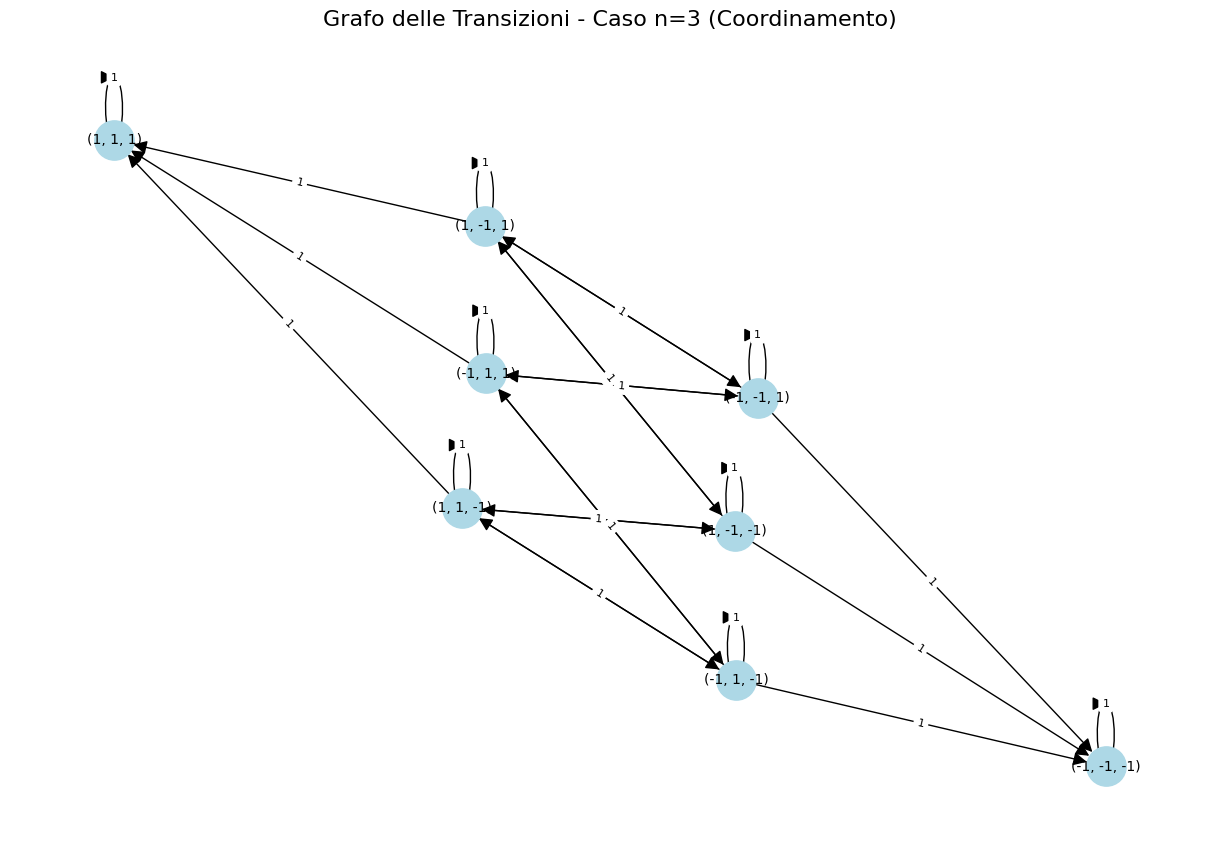
\includegraphics[width=0.8\textwidth]{graf1.png}
		\end{center}
		
		Figura 1: grafo con $n_1=3$\\
		I vari archi hanno probabilità 1 di essere percorsi poiché il giocatore che deve compiere l'azione é scelto casualmente.\\
		La soluzione dunque al limite é la seguente:
		\[
		\begin{cases}
			\frac{1}{2}, & \text{se } x = (+1, +1, +1), (-1, -1, -1) \\[5pt]
			0, & \text{negli altri casi} 
		\end{cases}
		\]
		Questo accade perché sono presenti due stati assorbenti.
		\newpage
		\item \textbf{b2}:
		\begin{center}
			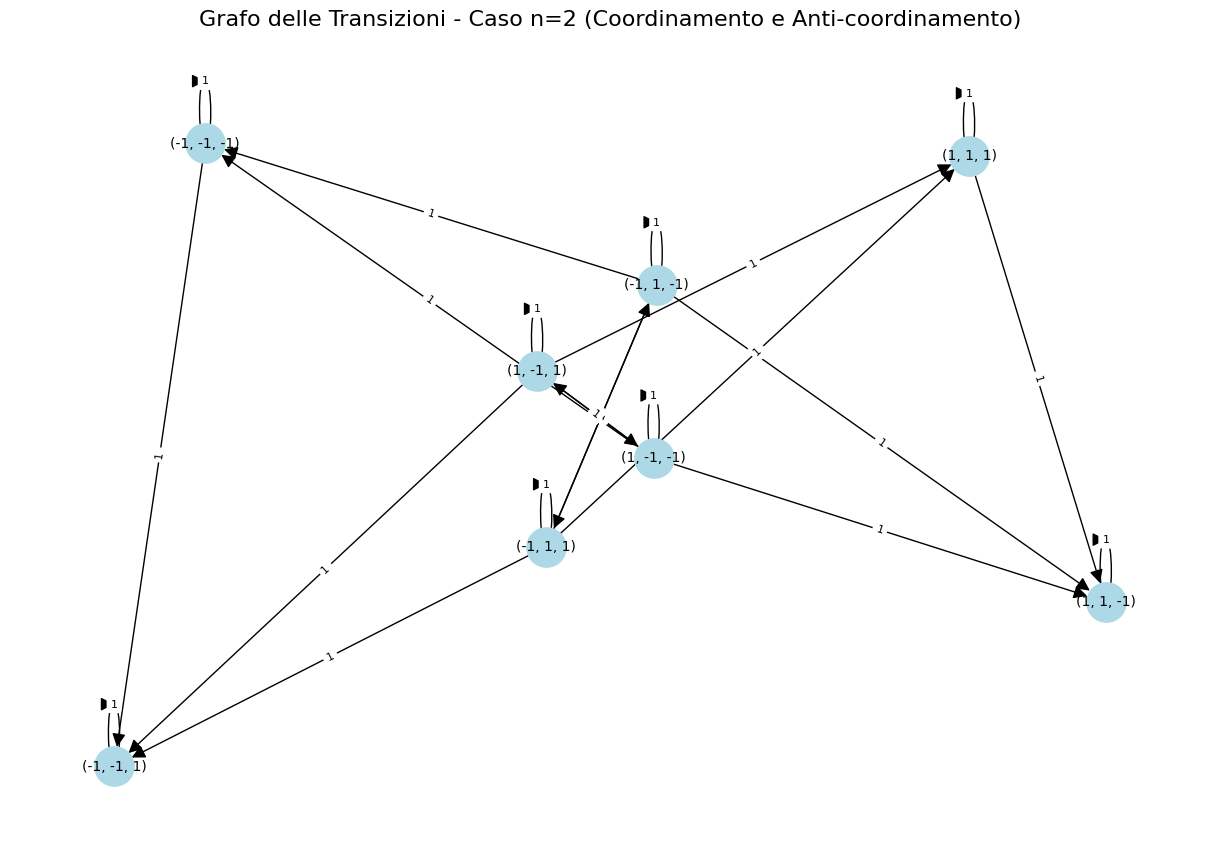
\includegraphics[width=0.8\textwidth]{graf2.png}
		\end{center}
		
		Figura 2: grafo con $n_1=2$\\
		I vari archi hanno probabilità 1 di essere percorsi poiché il giocatore che deve compiere l'azione é scelto casualmente.\\
		La soluzione dunque al limite é la seguente:
		\[
		\begin{cases}
			\frac{1}{2}, & \text{se } x = (+1, +1, -1), (-1, -1, +1) \\[5pt]
			0, & \text{negli altri casi} 
		\end{cases}
		\]
		Questo accade perché sono presenti due stati assorbenti.
	\end{itemize}
	\centering \textbf{Esercizio 3}\\
	\begin{itemize}
		\item \textbf{Punto a: }
		Abbiamo che il link $e_1$ ha costo $\omega_1$ mentre il link $e_2$ ha costo $\omega_2 + \frac{3}{2}x$.\\
		Di conseguenza ci basta risolvere il sistema\\
		\[
		\begin{cases}
			f_1 + f_2 = 1  \\
			\omega_1 = \omega_2 +\frac{3}{2}f_2 
		\end{cases}
		\]
		e otteniamo come risultato \\
		\[
		f_1=1-\frac{2}{3}(\omega_1-\omega_2)
		\]
		\[
		f_2=\frac{2}{3}(\omega_1-\omega_2)
		\]
		\item \textbf{Punto b: }
		Il flusso $f_1$ dipende da $\omega_1$ e $\omega_2$:
		\[
		f_1 =
		\begin{cases} 
			1 - \frac{2}{3} (\omega_1 - \omega_2), & \text{se } \omega_1 - \omega_2 \leq \frac{3}{2}, \\
			0, & \text{se } \omega_2 - \omega_1 > \frac{3}{2}.
		\end{cases}
		\]
		
		L'incasso del gestore 1 è quindi:
		\[
		u_1(\omega_1, \omega_2) = \omega_1 f_1.
		\]
		
		\textbf{Caso} $\omega_1 - \omega_2 \leq \frac{3}{2}$:
		Sostituendo $f_1 = 1 - \frac{2}{3} (\omega_1 - \omega_2)$ nell'incasso:
		\[
		u_1(\omega_1, \omega_2) = \omega_1 \left( 1 - \frac{2}{3} (\omega_1 - \omega_2) \right) 
		= \omega_1 - \frac{2}{3} \omega_1^2 + \frac{2}{3} \omega_1 \omega_2.
		\]
		
		Deriviamo rispetto a $\omega_1$ e poniamo la derivata pari a zero:
		\[
		\frac{\partial u_1}{\partial \omega_1} = 1 - \frac{4}{3} \omega_1 + \frac{2}{3} \omega_2 = 0.
		\]
		
		Risolvendo:
		\[
		\omega_1 = \frac{3 + 2 \omega_2}{4}.
		\]
		Il flusso $f_2$ dipende da $\omega_1$ e $\omega_2$:
		\[
		f_2 =
		\begin{cases} 
			\frac{2}{3} (\omega_1 - \omega_2), & \text{se } \omega_1 - \omega_2 > 0, \\
			0, & \text{se } \omega_2 - \omega_1 > 0.
		\end{cases}
		\]
		
		L'incasso del gestore 2 è quindi:
		\[
		u_2(\omega_1, \omega_2) = \omega_2 f_2.
		\]
		
		\textbf{Caso} $\omega_1 - \omega_2 >0$:
		Sostituendo $f_2 = \frac{2}{3} (\omega_1 - \omega_2)$ nell'incasso:
		\[
		u_2(\omega_1, \omega_2) = \omega_2 \left(  \frac{2}{3} (\omega_1 - \omega_2) \right) 
		=  - \frac{2}{3} \omega_2^2 + \frac{2}{3} \omega_1 \omega_2.
		\]
		
		Deriviamo rispetto a $\omega_2$ e poniamo la derivata pari a zero:
		\[
		\frac{\partial u_2}{\partial \omega_2} = - \frac{4}{3} \omega_2 + \frac{2}{3} \omega_1 = 0.
		\]
		
		Risolvendo:
		\[
		\omega_2 = \frac{ \omega_1}{2}.
		\]
		
		Le funzioni di best response sono dunque:
		\[
		B_1(\omega_2)=\frac{3 + 2 \omega_2}{4}
		\]
		\[
		B_2(\omega_1)=\frac{ \omega_1}{2}
		\]
		\item \textbf{Punto c: }
		Sostituendo $\omega_2^* = B_2(\omega_1^*) = \frac{\omega_1^*}{2}$ in $\omega_1^* = B_1(\omega_2^*)$:
		\[
		\omega_1^* = \frac{3 + 2\omega_2^*}{4}.
		\]
		
		Sostituiamo $\omega_2^* = \frac{\omega_1^*}{2}$:
		\[
		\omega_1^* = \frac{3 + 2\left(\frac{\omega_1^*}{2}\right)}{4}.
		\]
		
		Semplifichiamo:
		\[
		\omega_1^* = \frac{3 + \omega_1^*}{4}.
		\]
		
		Moltiplichiamo per 4:
		\[
		4\omega_1^* = 3 + \omega_1^*.
		\]
		
		Portiamo $\omega_1^*$ a sinistra:
		\[
		3\omega_1^* = 3 \implies \omega_1^* = 1.
		\]
		
		Ora sostituiamo $\omega_1^* = 1$ in $\omega_2^* = \frac{\omega_1^*}{2}$:
		\[
		\omega_2^* = \frac{1}{2}.
		\]
		
	\end{itemize}
	
\end{document}